\documentclass{article}
\usepackage{amsmath}
\usepackage{amssymb}
\usepackage[a4paper, top=25mm, bottom=25mm, left=25mm, right=25mm]{geometry}
\usepackage{pgfplots}
\usepackage{mathtools}
\pgfplotsset{compat=1.18}
\usepgfplotslibrary{fillbetween}
\usepackage{comment}
\usepackage[utf8]{inputenc}
\usepackage[T1]{fontenc}
\usepackage{parskip}

\begin{document}

\large

\begin{center}
{\huge MAT123 12.12.2025}
\end{center}

\vspace{1em}

{\setlength{\parindent}{1em} \Large
\indent \textbf{QUESTIONS}
}

\textbf{Q1.} Evaluate $\displaystyle\int\frac{2x^2+3}{x^2(4x^2+9)}\,dx$.

\textbf{Q2.} Calculate $\displaystyle\int_0^\infty\frac{x^2+x}{(x^2+1)^2}\,dx$.

\textbf{Q3.} Calculate $\displaystyle\int_0^{-2\pi}\sin(\theta)\cdot (\theta+\pi)^{\tfrac13}\cdot\arctan(\theta+\pi)\,d\theta$.

\textbf{Q4.} Evaluate $\displaystyle\int\frac1{3-2\cos x+\sin x}\,dx$.

\textbf{Q5.} Evaluate $\displaystyle\int_0^{\pi/2}\frac{\sin(2x)}{(a\sin^2x+b\cos^2x)^2}\,dx$, where $a, b >0$.

\textbf{Q6.} Find the area of the region bounded between $x=6-y^2$, $x=y$, and $y\geq1$.

\textbf{Q7.} Find the length of the graph of the function $y=\ln(1-x^2),\:0\leq x\leq1/2$.

\textbf{Q8.} What values of $p$ have the following property: The area of the region between the curve $y=x^{-p}, 1\leq x\leq\infty$, and the $x$-axis is infinite but the volume of the solid generated by revolving the region about the $x$-axis is finite. 

\textbf{Q9.} The graph of the equation $x^{2/3}+y^{2/3}=1$ is an astroid (\textit{see figure below}). Find the area of the surface generated by revolving the curve about the $x$-axis.

\begin{center}
\begin{tikzpicture}
  \begin{axis}[
    axis lines = center,
    axis equal image,
    xlabel = $x$, ylabel = $y$,
    domain=-2:2,
    samples=500,
    ymin=-1.1, ymax=1.1,
    xmin=-1.1, xmax=1.1,
    enlargelimits=true,
    clip=true,
    axis line style={->},
    scale=1.4,
    smooth,
    xtick={-1,1},
    ytick={-1,1},
    ]
    \addplot[blue, thick] {(1-x^(2/3))^(3/2)};
    \addplot[blue, thick] {-(1-x^(2/3))^(3/2)};
    \addplot[blue, thick] {(1-(-x)^(2/3))^(3/2)};
    \addplot[blue, thick] {-(1-(-x)^(2/3))^(3/2)};
    
  \end{axis}
\end{tikzpicture}
\end{center}

\newpage

{\setlength{\parindent}{1em} \Large
\indent \textbf{ANSWERS}
}

\textbf{Q1.} Use partial fraction decomposition.

Since the denominator contains a repeated linear factor \(x^2\) and an irreducible quadratic factor \(4x^2+9\), we write
\[
\frac{2x^2+3}{x^2(4x^2+9)}
= \frac{A}{x}+\frac{B}{x^2}+\frac{Cx+D}{4x^2+9}.
\]

Equate the denominator of each fraction. After we equate, we obtain these numerators:
\[
2x^2+3 = A x(4x^2+9)+B(4x^2+9)+(Cx+D)x^2.
\]

Compare coefficients. Equating coefficients of like powers of \(x\), we get
\[
A=0,\quad B=\frac13,\quad C=0,\quad D=\frac23.
\]

Rewrite the integrand. Substituting these values gives
\[
\frac{2x^2+3}{x^2(4x^2+9)}
= \frac{1}{3x^2}+\frac{2}{3(4x^2+9)}.
\]

Integrate term by term. The first integral is easy.
\begin{equation}
\int \frac{1}{3x^2}\,dx = -\frac{1}{3x}+c_1,
\end{equation}

To evaluate the second integral, we need to put it in a form that we can evaluate using standard integrals.

\[
\int \frac{2}{3(4x^2+9)}\,dx
= \frac{2}{3}\int \frac{1}{4x^2+9}\,dx= \frac{2}{3}\cdot \frac{1}{4}\int \frac{1}{x^2+\left(\frac{3}{2}\right)^2}\,dx= \frac{1}{6}\int \frac{1}{x^2+\left(\frac{3}{2}\right)^2}\,dx
\]

\[
\text{Let } x=\frac{3u}{2}\quad \Rightarrow \quad dx=\frac32\,du
\]

\begin{equation}
= \frac{1}{6}\int \frac{1}{\left(\frac{3}{2}\right)^2(u^2+1)}\cdot \frac32\,du=\frac19\int\frac1{u^2+1}\,du
= \frac{1}{9}\tan^{-1}(u)
= \frac{1}{9}\tan^{-1}\!\left(\frac{2x}{3}\right)+c_2
\end{equation}

Combining $(1)$ and $(2)$, we get the following.
\[
\boxed{\int \frac{2x^2+3}{x^2(4x^2+9)}\,dx
= -\frac{1}{3x}+\frac{1}{9}\tan^{-1}\!\left(\frac{2x}{3}\right)+C}
\]

\vspace{1em}

\newpage

\textbf{Q2.} Use partial fraction decomposition.
\[
\frac{x^2+x}{(x^2+1)^2}
= \frac{Ax+B}{x^2+1}+\frac{Cx+D}{(x^2+1)^2}.
\]

Equate the denominator of each fraction. After we equate, we obtain these numerators:, we get
\[
x^2+x = (Ax+B)(x^2+1)+(Cx+D).
\]

Expanding,
\[
x^2+x = Ax^3+Ax+Bx^2+B+Cx+D.
\]

Comparing coefficients yields
\[
A=0,\quad B=1,\quad C=1,\quad D=-1.
\]

Hence,
\[
\int\frac{x^2+x}{(x^2+1)^2}\,dx
=\int\frac{1}{x^2+1}\,dx+\int\frac{x-1}{(x^2+1)^2}\,dx.
\]

Now, integrate term by term. The first integral appears to be an improper integral of Type I. Take the limit and then evaluate the integral.
\begin{align}\nonumber
\int_0^\infty\frac{1}{x^2+1}\,dx &=\lim_{R\to\infty}\int_0^R\frac1{x^2+1}\,dx=\lim_{R\to\infty}\arctan x\bigg|_0^R=\lim_{R\to\infty}(\arctan R -\arctan0)\\&=\frac\pi2-0=\frac\pi2
\end{align}

Evaluate the second integral by using a trigonometric substitution. Now, we can ignore the limits of integration. After we return to the variable $x$, we must consider the upper and lower limits.

\[
\text{Let } x=\tan\theta \quad \Rightarrow \quad dx=\sec^2\theta\,d\theta
\]

\begin{align*}
\int \frac{x-1}{(x^2+1)^2}\,dx
&= \int \frac{\tan\theta-1}{\sec^4\theta}\,\sec^2\theta\,d\theta=\int (\tan\theta-1)\cos^2\theta\,d\theta\\&=\int \left(\sin\theta\cos\theta-\cos^2\theta\right)d\theta=\int\frac12\sin2\theta\,d\theta-\int \frac{1+\cos 2\theta}{2}\,d\theta\\&=-\frac14\cos2\theta-\frac\theta2-\frac{\sin2\theta}4+C
\end{align*}

Recall the substitution $x=\tan\theta$, then $\arctan x=\theta$.

\[
-\frac14\cos(2\arctan x)-\frac{\arctan x}2-\frac{\sin(2\arctan x)}4+C
\]

We evaluated the indefinite integral. However, the original integral we want to evaluate is an improper integral of Type I. Therefore, we take the limit.

\begin{align}\nonumber\int_0^\infty\frac{x-1}{(x^2+1)^2}\,dx&=\lim_{R\to\infty}\left[
-\frac14\cos(2\arctan x)-\frac{\arctan x}2-\frac{\sin(2\arctan x)}4\right]_0^R\\&=\nonumber\left(-\frac14\cos(\pi)-\frac\pi4-\frac{\sin\pi}4\right)-\left(-\frac14\cos0-0-\frac{\sin0}2\right)\\&=\left(\frac14-\frac\pi4-0\right)-\left(-\frac14-0-0\right)=\frac12-\frac\pi4
\end{align}

Combine $(3)$ and $(4)$.

\[\boxed{\frac12+\frac\pi4}\]

\vspace{1em}

\textbf{Q3.} Let $u = \theta + \pi \implies du = d\theta$. Then $\sin(\theta) = \sin(u-\pi) = -\sin(u)$.

When $\theta=0$, $u=\pi$, and when $\theta=-2\pi$, $u=-\pi$. So the integral becomes
\begin{align*}
\int_0^{-2\pi} \sin(\theta) \cdot(\theta+\pi)^{1/3} \cdot \arctan(\theta+\pi)\,d\theta
&= \int_\pi^{-\pi} -\sin(u)\cdot u^{1/3} \cdot\arctan(u)\,du
\\&= \int_{- \pi}^{\pi} \sin(u)\cdot u^{1/3} \cdot\arctan(u)\,du.
\end{align*}

The integrand $f(u) = \sin(u) \cdot u^{1/3}\cdot \arctan(u)$ is an odd function because each factor is odd. Therefore, by the property of integrals of odd functions over symmetric limits,
\[
\int_{- \pi}^{\pi} f(u)\,du = 0.
\]

\[
\boxed{0}
\]

\vspace{1em}

\textbf{Q4.} Use the Weierstrass substitution (tangent half-angle substitution):
\[
t = \tan\frac{x}{2} \implies dx = \frac{2\, dt}{1+t^2},\quad \sin x = \frac{2t}{1+t^2},\quad \cos x = \frac{1-t^2}{1+t^2}.
\]

Then
\[
3 - 2\cos x + \sin x = \frac{5 t^2 + 2 t + 1}{1+t^2}, \quad dx = \frac{2\, dt}{1+t^2}.
\]

So the integral becomes
\[
\int \frac{dx}{3-2\cos x + \sin x} = \int \frac{2\, dt}{5 t^2 + 2 t + 1}.
\]

Next, we complete the square in the denominator:

\[
5 t^2 + 2 t + 1 = 5\left(t^2 + \frac{2}{5} t + \frac{1}{5}\right) = 5\left(\left(t + \frac{1}{5}\right)^2 + \frac{4}{25}\right).
\]

Factor out \(\frac{4}{25}\) to get a $1$ inside the parentheses:

\[
5\left(\left(t + \frac{1}{5}\right)^2 + \frac{4}{25}\right) = 5 \cdot \frac{4}{25} \left( \frac{25}{4}\left(t + \frac{1}{5}\right)^2 + 1 \right) = \frac{4}{5} \left( \left(\frac{5}{2} t + \frac{1}{2}\right)^2 + 1 \right).
\]

So the integral becomes

\[
\int \frac{2\, dt}{5 t^2 + 2 t + 1} = \int \frac{2\, dt}{\frac{4}{5} \left( \left(\frac{5}{2} t + \frac{1}{2}\right)^2 + 1 \right)} = \frac{5}{2} \int \frac{dt}{\left(\frac{5}{2} t + \frac{1}{2}\right)^2 + 1}.
\]

Finally, let

\[
u = \frac{5}{2} t + \frac{1}{2} \implies du = \frac{5}{2} dt \implies dt = \frac{2}{5} du,
\]

so the integral becomes

\[
\frac{5}{2} \int \frac{dt}{\left(\frac{5}{2} t + \frac{1}{2}\right)^2 + 1} = \frac{5}{2} \cdot \frac{2}{5} \int \frac{du}{u^2 + 1} = \int \frac{du}{u^2 + 1} = \arctan(u) + C.
\]

Substitute \(u = \frac{5}{2} t + \frac{1}{2}\) and \(t = \tan\frac{x}{2}\) back.

\[
\boxed{\arctan\left(\frac{5}{2} \tan\frac{x}{2} + \frac{1}{2}\right) + C}
\]

\vspace{1em}

\textbf{Q5.} Let $u = \sin x \implies du = \cos x \, dx$. Then
\[
\sin 2x = 2 \sin x \cos x = 2 u \sqrt{1-u^2}, \quad dx = \frac{du}{\sqrt{1-u^2}}.
\]
\[
x=\frac\pi2\implies u=1,\qquad x=0\implies u=0
\]

So the integral becomes
\[
I = \int_0^1 \frac{2 u \sqrt{1-u^2}}{(a u^2 + b (1-u^2))^2} \cdot \frac{du}{\sqrt{1-u^2}} = \int_0^1 \frac{2 u}{((a-b) u^2 + b)^2} \, du.
\]

Let $v= (a-b)u^2 + b \implies dv = 2u(a-b)\,du$, and $u=1\implies w=b,\:u=0\implies w=a$. So
\[
I = \frac{1}{a-b} \int_b^a \frac{dv}{v^2} = \frac{1}{a-b} \left[-\frac{1}{v}\right]_b^a=\frac{1}{a-b}\left(\frac1b-\frac1a\right)=\boxed{\frac{1}{ab}}.
\]

\newpage

\textbf{Q6.}

\begin{center}
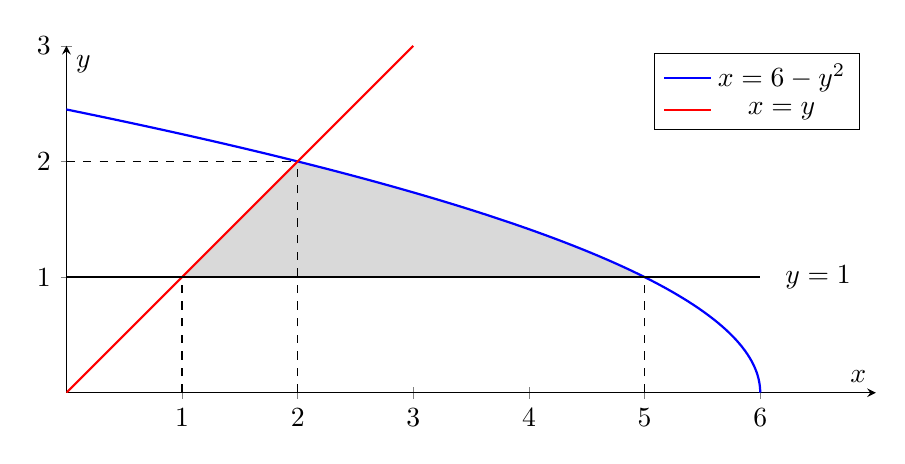
\begin{tikzpicture}
\begin{axis}[
    axis lines=middle,
    axis equal image,
    xlabel={$x$},
    ylabel={$y$},
    xmin=0, xmax=7,
    ymin=0, ymax=3,
    xtick={0,1,2,3,4,5,6},
    ytick={0,1,2,3},
    samples=100,
    domain=0:3,
    clip=true,
    scale=1.5,
]

\addplot [name path=A, blue, thick, domain=0:3] ({6 - x^2}, x);
\addlegendentry{$x=6-y^2$}

\addplot [name path=B, red, thick, domain=0:3] {x};
\addlegendentry{$x=y$}

\addplot [name path=lower, black, thick, domain=0:6] {1};
    \draw[dashed] (1,0)--(1,1);
    \draw[dashed] (5,0)--(5,1);
    \draw[dashed] (2,0)--(2,2);
    \draw[dashed] (0,2)--(2,2);


\addplot [
    thick,
    color=gray,
    fill=gray, 
    fill opacity=0.3
] fill between[
    of=lower and B,
    soft clip={domain=1:2},
];

\addplot [
    thick,
    color=gray,
    fill=gray, 
    fill opacity=0.3
] fill between[
    of=lower and A,
    soft clip={domain=2:5},
];

\node at (6.5,1) {$y=1$};

\end{axis}


\end{tikzpicture}
\end{center}

Method 1: Integrate with respect to $y$.

Horizontal distance: $x_{\text{right}} - x_{\text{left}} = (6-y^2) - y$.

\[
A = \int_1^2 (6 - y^2 - y) \, dy = \int_1^2 6\, dy - \int_1^2 y^2\, dy - \int_1^2 y\, dy
= 6 - \frac{7}{3} - \frac{3}{2} = \boxed{\frac{13}6}
\]

\vspace{1em}

Method 2: Integrate with respect to $x$.

Express curves as functions of $x$: $y = \sqrt{6-x}$ and $y = x$.

For $1\leq x \leq 2$, the upper function is $y=x$. Meanwhile, the lower function is $y=1$. For $2\leq x\leq 5$, these are $y=\sqrt{6-x}$ and $y=1$, respectively. Therefore, we take two integrals.

\begin{align*}\int_1^2(x-1)\,dx+\int_2^5(\sqrt{6-x}-1)\,dx&=\left[\frac{x^2}2-x\right]_1^2+\left[-\frac23(6-x)^{3/2}-x\right]_2^5\\&=\left(0-\left(\frac12-1\right)\right)+\left(\left(-\frac23-5\right)-\left(-\frac{16}3-2\right)\right)\\&=\frac12+\frac53=\boxed{\frac{13}6}\end{align*}

\vspace{1em}

\textbf{Q7.} The arc length formula is
\[
L = \int_0^{1/2} \sqrt{1 + \left(\frac{dy}{dx}\right)^2} \, dx.
\]

\[
y = \ln(1-x^2) \implies \frac{dy}{dx} = \frac{-2x}{1-x^2}
\]

\[
1 + \left(\frac{dy}{dx}\right)^2 = 1 + \frac{4x^2}{(1-x^2)^2} = \frac{(1-x^2)^2 + 4x^2}{(1-x^2)^2} = \frac{(1+x^2)^2}{(1-x^2)^2} = \left(\frac{1+x^2}{1-x^2}\right)^2
\]

Hence,
\[
L = \int_0^{1/2} \frac{1+x^2}{1-x^2} \, dx.
\]
Split the fraction.
\[
\frac{1+x^2}{1-x^2} = -1 + \frac{2}{1-x^2}
\]

Thus, the integral becomes
\[
L = \int_0^{1/2} \left(-1 + \frac{2}{1-x^2}\right) dx = \int_0^{1/2} (-1) \, dx + \int_0^{1/2} \frac{2}{1-x^2} \, dx.
\]

The first integral is simple.
\begin{equation}
\int_0^{1/2} (-1) \, dx = -\frac{1}{2}
\end{equation}

For the second integral, factor using partial fractions.
\[
\frac2{1-x^2} = \frac{1}{1-x} + \frac{1}{1+x} 
\]

\[
\int_0^{1/2} \frac{2}{1-x^2} \, dx = \int_0^{1/2} \frac{1}{1-x} \, dx + \int_0^{1/2} \frac{1}{1+x} \, dx
\]

\text{Integrate each term.}
\begin{equation}
\int_0^{1/2} \frac{1}{1-x} \, dx = -\ln|1-x| \Big|_0^{1/2} = \ln1-\ln\frac{1}{2} = \ln 2
\end{equation}

\begin{equation}
\int_0^{1/2} \frac{1}{1+x} \, dx = \ln|1+x| \Big|_0^{1/2} = \ln \frac{3}{2}-\ln1=\ln\frac32
\end{equation}

Combine $(5)$, $(6)$, and $(7)$.
\[
L = -\frac{1}{2} + \ln 2 + \ln \frac{3}{2} = -\frac{1}{2} + \ln 3 - \ln 2 + \ln 2 = \ln 3 - \frac12
\]

\[
\boxed{L = \ln 3-\frac12}
\]

\vspace{1em}

\textbf{Q8.} The area is
\[
A = \int_1^\infty x^{-p} \, dx.
\]

For $p \neq 1$, we have
\[
\int_1^\infty x^{-p} \, dx = \lim_{b \to \infty} \frac{x^{1-p}}{1-p} \Big|_1^b = \lim_{b \to \infty} \frac{b^{1-p}-1}{1-p}.
\]

\begin{itemize}
    \item If $p < 1$, then $1-p>0$ and $b^{1-p} \to \infty$, so the integral diverges.
    \item If $p > 1$, then $1-p<0$ and $b^{1-p} \to 0$, so the integral converges.
    \item If $p = 1$, $\displaystyle\int_1^\infty x^{-1} dx = \int_1^\infty \frac{dx}{x} = \lim_{R\to\infty}(\ln R-\ln1)=\infty$.
\end{itemize}

Condition for infinite area: $p \leq 1$.

The volume generated by revolving around the $x$-axis is
\[
V = \pi \int_1^\infty (x^{-p})^2 \, dx = \pi \int_1^\infty x^{-2p} \, dx.
\]

For $2p \neq 1$,
\[
\pi\int_1^\infty x^{-2p} \, dx = \pi\lim_{b \to \infty} \frac{x^{1-2p}}{1-2p} \Big|_1^b = \pi\lim_{b \to \infty} \frac{b^{1-2p}-1}{1-2p}.
\]

\begin{itemize}
    \item If $2p > 1 \implies p > \frac{1}{2}$, then $1-2p < 0$ and $b^{1-2p} \to 0$, so the integral converges.
    \item If $2p < 1 \implies p <\frac{1}{2}$, the integral diverges.
    \item If $2p=1 \implies p =\frac{1}{2}$, the integral diverges because $\displaystyle\int_1^\infty\frac1x\,dx=\infty$.
\end{itemize}

Condition for finite volume: $p > \frac{1}{2}$.

Combine conditions.

\[
p \le 1 \quad \text{(area is infinite)}, \qquad p > \frac{1}{2} \quad \text{(volume is finite)}
\]

\[
\boxed{\frac{1}{2} < p \le 1}
\]

\vspace{1em}

\textbf{Q9.} We may consider the curves in Quadrant I and II. Then it is redundant to use the lower part since the rotated curves are the same.
Solve for $y$.
\[
y = (1 - x^{2/3})^{3/2}, \quad x \in [-1,1]
\]

Surface area formula:
\[
S = 2\pi \int_{-1}^1 y \sqrt{1 + \left(\frac{dy}{dx}\right)^2} \, dx
\]

Compute $dy/dx$.
\[
\frac{dy}{dx} = \frac{3}{2} (1 - x^{2/3})^{1/2} \cdot \left(-\frac{2}{3} x^{-1/3}\right) = - x^{-1/3} (1 - x^{2/3})^{1/2}
\]

\[
\left(\frac{dy}{dx}\right)^2 = x^{-2/3} (1 - x^{2/3})
\]

\[
\sqrt{1 + \left(\frac{dy}{dx}\right)^2} = \sqrt{1 + x^{-2/3}(1 - x^{2/3})} = \sqrt{x^{-2/3}} = \left|x^{-1/3}\right|
\]

Set up the integral.
\[
S = 2\pi \int_{-1}^1 (1 - x^{2/3})^{3/2} \cdot \left|x^{-1/3}\right|\,dx
\]

The expression $\left|x^{-2/3}\right|$ is positive for $x>0$ and negative for $x<0$. We may rewrite this integral as follows.
\begin{align*}
S &= 2\pi \int_{-1}^1 (1 - x^{2/3})^{3/2} \cdot \left|x^{-1/3}\right|\,dx\\&=2\pi \int_{-1}^0(1-x^{2/3})^{3/2}\left(-x^{-1/3}\right)\,dx+2\pi \int_0^1(1-x^{2/3})^{3/2}\left(x^{-1/3}\right)\,dx\\&=4\pi \int_0^1(1-x^{2/3})^{3/2}x^{-1/3}\,dx\qquad\left[\text{symmetry property}\right]
\end{align*}

Let $u = x^{2/3} \implies du = \frac23 x^{-1/3}\,
dx$. Then
\[
x^{-1/3} dx = \frac{3}{2} du, \quad (1 - x^{2/3})^{3/2} = (1 - u)^{3/2}.
\]

\[
S = 4\pi \int_0^1 (1-u)^{3/2} \cdot \frac{3}{2}\,du = 6\pi \int_0^1 (1-u)^{3/2}\,du
\]

Integrate.
\[
S=6\pi\int_0^1 (1-u)^{3/2}\,du=6\pi\cdot\left[-\frac25\left(1-u\right)^{5/2}\right]_0^1=6\pi\left[0-\left(-\frac25\right)\right]=\boxed{\frac{12\pi}5}
\]

\end{document}